%%% CSE 4317 DDS - WORKED EXAMPLE (Autonomous Ground Robot)
%%% Structure follows IEEE Std 1016-2009 (Software Design Descriptions).
\documentclass[11pt,letterpaper]{article}
\usepackage[margin=1.0in]{geometry}
\usepackage[T1]{fontenc}
\usepackage[bitstream-charter]{mathdesign}
\usepackage[latin1]{inputenc}
\usepackage{amsmath}\usepackage{xcolor}\usepackage{cite}\usepackage{hyphenat}
\usepackage{graphicx}\usepackage{float}\usepackage{subfigure}\usepackage{sectsty}
\usepackage[compact]{titlesec}\usepackage[tablegrid]{vhistory}\usepackage{pbox}\usepackage{longtable}
\allsectionsfont{\color{accentcolor}\scshape\selectfont}
\definecolor{accentcolor}{rgb}{0.0,0.0,0.5}
\newcommand{\teamname}{Team Trailblazer}
\newcommand{\productname}{TerraScout Autonomous Ground Rover}
\newcommand{\coursename}{CSE 4317: Senior Design II}
\newcommand{\semester}{Spring 2027}
\newcommand{\docname}{Detailed Design Specification}
\newcommand{\department}{Department of Computer Science \& Engineering}
\newcommand{\university}{The University of Texas at Arlington}
\newcommand{\authors}{Alan Turing \\ Grace Hopper \\ John Von Neumann \\ Ada Lovelace \\ Charles Babbage}
\usepackage{fancyhdr}\pagestyle{fancy}\usepackage{lastpage}
\lhead{}\chead{}\rhead{}\lfoot{\footnotesize \teamname \ - \semester}\cfoot{}
\rfoot{\footnotesize page \thepage\ of \pageref{LastPage}}
\renewcommand{\headrulewidth}{0.0pt}\renewcommand{\footrulewidth}{0.4pt}
\usepackage[runin]{abstract}\abslabeldelim{\quad}\setlength{\abstitleskip}{-10pt}
\renewcommand{\abstractname}{}\renewcommand{\abstracttextfont}{\color{accentcolor} \small \slshape}

\begin{document}
{\centering \huge \color{accentcolor} \sc \textbf{\department \\ \university} \par}
\vspace{1 in}
{\centering \huge \color{accentcolor} \sc \textbf{\docname \\ \coursename \\ \semester} \par}
\vspace{0.5 in}
\begin{figure}[h!]\centering
\includegraphics[width=0.60\textwidth]{images/test_image}\end{figure}
\vspace{0.5 in}
{\centering \huge \color{accentcolor} \sc \textbf{\teamname \\ \productname} \par}
\vspace{0.5 in}
{\centering \large \sc \textbf{\authors} \par}
\newpage

\begin{versionhistory}
  \vhEntry{0.1}{01.20.2027}{CB}{document creation}
  \vhEntry{1.0}{02.05.2027}{AT|GH|CB}{official release}
\end{versionhistory}
\newpage
\setcounter{tocdepth}{2}\tableofcontents
\newpage

\section{Introduction}
This DDS gives the implementation-level design of \productname\ as a Software Design
Description per IEEE Std 1016-2009 \cite{IEEE1016}. It builds on the SRS
(requirements) and ADS (architecture, three layers X/Y/Z), adding hardware,
software, data, and algorithm detail. Representative subsystems are detailed below.

\section{Design Stakeholders \& Concerns}
Implementers, integrators, testers, and maintainers. Concerns: composition,
interfaces, data structures, timing/state behavior, algorithms, and the hardware/OS
resources each subsystem requires.

\section{Design Viewpoints}
Each subsystem is described through the relevant IEEE 1016 viewpoints: Context,
Composition, Information (data structures), Interface, Interaction \& State,
Algorithm, and Resource (hardware/OS/dependencies/languages). Viewpoints that do
not apply are omitted.

\section{System Overview}
\begin{figure}[h!]\centering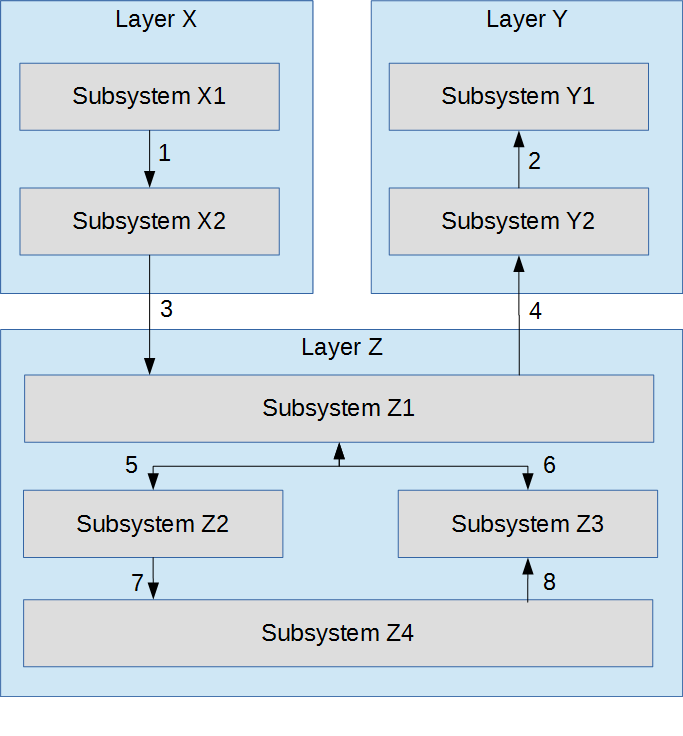
\includegraphics[width=0.9\textwidth]{images/data_flow}
\caption{System architecture carried forward from the ADS}\end{figure}
Compute runs on an NVIDIA Jetson-class module (Ubuntu, ROS~2); platform subsystems
are STM32 microcontrollers on a CAN bus. The ground-station app runs on the
operator laptop.

\section{X Layer Subsystems --- Perception \& Sensing}
\subsection{Layer Resources}
\textbf{Hardware:} RGB CSI camera, USB thermal camera, RTK-GNSS receiver, IMU.
\textbf{OS:} Ubuntu 22.04 on the compute module. \textbf{Dependencies:} ROS~2,
OpenCV, GNSS driver.
\subsection{X.Imaging}
\textbf{Context/Composition:} a ROS~2 node wrapping both cameras and a hardware
trigger. \textbf{Information:} \texttt{Frame\{stamp, pose, rgb[H][W][3],
thermal[h][w]\}}. \textbf{Interface (\#01):} subscribes \texttt{/trigger},
\texttt{/pose}; publishes \texttt{/frames}. \textbf{Algorithm/State:} on trigger,
grab both cameras, attach nearest-in-time pose, publish. \textbf{Resource:} C++ for
the driver; $\sim$8\,W. \textbf{Rationale:} hardware trigger removes RGB/thermal
skew (AD-02); C++ meets frame-rate.

\section{Y Layer Subsystems --- Autonomy \& Compute}
\subsection{Layer Resources}
\textbf{OS/Deps:} Ubuntu, ROS~2, Nav2 stack, PyTorch (inference), FastAPI (ground
station). \textbf{Languages:} C++ (navigation), Python (detection, server).
\subsection{Y.Navigation}
\textbf{Composition:} Nav2-based planner + controller nodes.
\textbf{Interface (\#03):} in \texttt{/pose}, \texttt{/waypoints},
\texttt{/proximity}; out \texttt{/cmd\_vel}. \textbf{Algorithm:} pure-pursuit path
following with a costmap for obstacle avoidance; cross-track error held $\leq$0.5\,m
(FR-01). \textbf{State:} \texttt{PLAN$\rightarrow$FOLLOW$\rightarrow$AVOID$\rightarrow$ARRIVED}.
\textbf{Rationale:} Nav2 reuse over a hand-written planner (AD-01).
\subsection{Y.FaultDetection}
\textbf{Composition:} a Python node loading a replaceable model artifact
(QA-01). \textbf{Information:} input \texttt{Frame}; output
\texttt{Detection\{class, confidence, pose, image\_ref\}}. \textbf{Interface:}
subscribes \texttt{/frames}; publishes \texttt{/detections}. \textbf{Algorithm:} a
lightweight CNN (MobileNet-class backbone) fine-tuned on the sponsor set; per-region
softmax over \{nominal, hotspot, soiling, crack\}; thresholded to meet PE-03.
\textbf{Resource:} GPU inference on the Jetson. \textbf{Rationale:} edge inference
per AD-02; model file swap keeps navigation untouched.
\subsection{Y.Mission \& Y.GroundStationServer}
\textbf{Y.Mission} runs the state machine (idle/patrol/capture/return/dock),
enforces FR-05 triggers (obstacle, SoC$\leq$20\%, link-loss$>$10\,s), and builds the
CSV+image report (FR-04). \textbf{Y.GroundStationServer} is a FastAPI service
terminating the TLS~1.3 WebSocket (SE-01, EI-01), streaming telemetry at 2\,Hz and
serving reports.

\section{Z Layer Subsystems --- Mobility \& Power}
\subsection{Layer Resources}
\textbf{Hardware:} 4$\times$brushless motors + CAN motor controllers, 24\,V LiFePO4
battery + BMS, STM32 microcontrollers. \textbf{Languages:} C (firmware).
\subsection{Z.Drive}
\textbf{Interface (\#04):} consumes \texttt{/cmd\_vel} bridged to CAN torque
commands; returns wheel odometry. \textbf{State:} a hardware E-stop line
de-energizes motor power independent of firmware (SA-01). \textbf{Algorithm:}
per-wheel PID velocity control. \textbf{Rationale:} hardware E-stop path is not
software-defeatable.
\subsection{Z.Power}
Reports state-of-charge from the BMS over CAN (drives FR-05); controls dock
charging contactor (EI-02).

\section{Requirements Traceability}
\begin{table}[H]\begin{center}\begin{tabular}{ | p{1.6cm} | p{5cm} | p{3.4cm} | p{1.6cm} |}\hline
\textbf{Req} & \textbf{Requirement (abbrev.)} & \textbf{Component} & \textbf{Iface} \\ \hline
FR-01 & Waypoint patrol & Y.Navigation & \#03 \\ \hline
FR-02 & Imagery capture & X.Imaging & \#01 \\ \hline
FR-03 & Fault detection & Y.FaultDetection & --- \\ \hline
FR-05 & Safe-stop/return & Y.Mission, Z.Power & \#04 \\ \hline
SA-01 & Emergency stop & Z.Drive (HW E-stop) & \#04 \\ \hline
SE-01 & Encrypted link & Y.GroundStationServer & \#01(GS) \\ \hline
\end{tabular}\end{center}\end{table}

\section{Appendix A}
Wiring schematic, CAN message catalog, and chassis CAD (STEP) are attached as
separate files in the closeout package.

\bibliographystyle{reference/IEEEtran_custom}
\bibliography{reference/refs}{}
\end{document}
